\documentclass[aps,prb,reprint,showkeys,superscriptaddress]{revtex4-1}
\usepackage{subcaption}
\captionsetup{justification   = raggedright,
              singlelinecheck = false}
\usepackage{bm,graphicx,tabularx,array,booktabs,dcolumn,xcolor,microtype,multirow,amscd,amsmath,amssymb,amsfonts,physics,siunitx}
\usepackage[version=4]{mhchem}
\usepackage[utf8]{inputenc}
\usepackage[T1]{fontenc}
\usepackage{txfonts}
\usepackage[normalem]{ulem}
\usepackage{mleftright}

%%% Definition of colors for personal remark %%%
\newcommand{\todo}[1]{\textcolor{red}{#1}}
\newcommand{\ant}[1]{\textcolor{orange}{#1}}
\newcommand{\trashant}[1]{\textcolor{orange}{\sout{#1}}}

\usepackage[
	colorlinks=true,
    citecolor=blue,
    linkcolor=blue,
    filecolor=blue,      
    urlcolor=blue,	
    breaklinks=true
	]{hyperref}
\urlstyle{same}

%============================================================%
%%% NEWCOMMANDS %%%
%============================================================%

%============================================================%
%%% NEWCOMMANDS %%%
% ============================================================%

%%% This latex gather all the latex commands that I use to facilitate the writing of electronic structure manuscript, report...
%%% You can import these commands by adding the following line in you .text
%%% %============================================================%
%%% NEWCOMMANDS %%%
% ============================================================%

%%% This latex gather all the latex commands that I use to facilitate the writing of electronic structure manuscript, report...
%%% You can import these commands by adding the following line in you .text
%%% %============================================================%
%%% NEWCOMMANDS %%%
% ============================================================%

%%% This latex gather all the latex commands that I use to facilitate the writing of electronic structure manuscript, report...
%%% You can import these commands by adding the following line in you .text
%%% \input{commands}

%%% Latin %%%

\newcommand{\ie}{\textit{i.e.}~}
\newcommand{\eg}{\textit{e.g.}~}
\newcommand{\etal}{\textit{et al.}~}

%%% Operators %%%

\newcommand{\hH}{\Hat{H}} % Hamiltonian operator
\newcommand{\HN}{\Hat{\mathnormal{H}}_{\text{N}}} % Normal ordered Hamiltonian
\newcommand{\Hsim}{\hat{\bar{H}}} % Similarity transformed Hamiltonian
\newcommand{\hC}{\Hat{C}} % CI operator
\newcommand{\hT}{\Hat{T}} % Cluster operator
\newcommand{\T}[1]{\Hat{\mathnormal{T}}_{#1}} % Cluster operator of a given excitation number
\newcommand{\hsig}{\Hat{\sigma}} % Unitary cluster operator
\newcommand{\hK}{\Hat{K}} % Anti-hermitian orbital rotation operator
\newcommand{\hS}{\Hat{S}} % Anti-hermitian CI coefficients rotation operator
\newcommand{\hP}[1]{\Hat{\mathnormal{P}}_{#1}} % Permutation operators

\newcommand{\hE}{\Hat{E}} % Spin averaged single excitation operator
\newcommand{\cre}[1]{a_{#1}^\dagger} % Creation operator
\newcommand{\ani}[1]{a_{#1}} % Annihilation operator
\newcommand{\bcre}[1]{b_{#1}^\dagger} % Boson creation operator
\newcommand{\bani}[1]{b_{#1}} % Boson annihilation operator

\newcommand{\com}[2]{\mleft[#1,#2 \mright]} % Commutator

%%% Wave functions %%%



%%% Matrix and tensor elements %%%

\newcommand{\oa}{O_{\alpha}}
\newcommand{\ob}{O_{\beta}}
\newcommand{\eri}[2]{\braket{#1}{#2}} % Electron repulsion integral physician notation
\newcommand{\ceri}[2]{\mleft(#1|#2\mright)} % Electron repulsion integral chemist notation
\newcommand{\dbi}[2]{\mel{#1}{}{#2}} % Double bar integral
\newcommand{\kron}[1]{\delta_{#1}} % Kronecker delta

%%% Matrix %%%

\newcommand{\FC}[1]{F_{#1}^{\text{C}}} % Core Fock matrix
\newcommand{\FA}[1]{F_{#1}^{\text{A}}} % Active Fock matrix

%%% Text acronyms and abbreviations %%%

\newcommand{\FCI}{\text{FCI}}
\newcommand{\HF}{\text{HF}}
\newcommand{\MCSCF}{\text{MCSCF}}
\newcommand{\occ}{\text{occ}}
\newcommand{\vir}{\text{vir}}


\newcommand{\SupInf}{\textcolor{blue}{Supporting Information}}



%%% Latin %%%

\newcommand{\ie}{\textit{i.e.}~}
\newcommand{\eg}{\textit{e.g.}~}
\newcommand{\etal}{\textit{et al.}~}

%%% Operators %%%

\newcommand{\hH}{\Hat{H}} % Hamiltonian operator
\newcommand{\HN}{\Hat{\mathnormal{H}}_{\text{N}}} % Normal ordered Hamiltonian
\newcommand{\Hsim}{\hat{\bar{H}}} % Similarity transformed Hamiltonian
\newcommand{\hC}{\Hat{C}} % CI operator
\newcommand{\hT}{\Hat{T}} % Cluster operator
\newcommand{\T}[1]{\Hat{\mathnormal{T}}_{#1}} % Cluster operator of a given excitation number
\newcommand{\hsig}{\Hat{\sigma}} % Unitary cluster operator
\newcommand{\hK}{\Hat{K}} % Anti-hermitian orbital rotation operator
\newcommand{\hS}{\Hat{S}} % Anti-hermitian CI coefficients rotation operator
\newcommand{\hP}[1]{\Hat{\mathnormal{P}}_{#1}} % Permutation operators

\newcommand{\hE}{\Hat{E}} % Spin averaged single excitation operator
\newcommand{\cre}[1]{a_{#1}^\dagger} % Creation operator
\newcommand{\ani}[1]{a_{#1}} % Annihilation operator
\newcommand{\bcre}[1]{b_{#1}^\dagger} % Boson creation operator
\newcommand{\bani}[1]{b_{#1}} % Boson annihilation operator

\newcommand{\com}[2]{\mleft[#1,#2 \mright]} % Commutator

%%% Wave functions %%%



%%% Matrix and tensor elements %%%

\newcommand{\oa}{O_{\alpha}}
\newcommand{\ob}{O_{\beta}}
\newcommand{\eri}[2]{\braket{#1}{#2}} % Electron repulsion integral physician notation
\newcommand{\ceri}[2]{\mleft(#1|#2\mright)} % Electron repulsion integral chemist notation
\newcommand{\dbi}[2]{\mel{#1}{}{#2}} % Double bar integral
\newcommand{\kron}[1]{\delta_{#1}} % Kronecker delta

%%% Matrix %%%

\newcommand{\FC}[1]{F_{#1}^{\text{C}}} % Core Fock matrix
\newcommand{\FA}[1]{F_{#1}^{\text{A}}} % Active Fock matrix

%%% Text acronyms and abbreviations %%%

\newcommand{\FCI}{\text{FCI}}
\newcommand{\HF}{\text{HF}}
\newcommand{\MCSCF}{\text{MCSCF}}
\newcommand{\occ}{\text{occ}}
\newcommand{\vir}{\text{vir}}


\newcommand{\SupInf}{\textcolor{blue}{Supporting Information}}



%%% Latin %%%

\newcommand{\ie}{\textit{i.e.}~}
\newcommand{\eg}{\textit{e.g.}~}
\newcommand{\etal}{\textit{et al.}~}

%%% Operators %%%

\newcommand{\hH}{\Hat{H}} % Hamiltonian operator
\newcommand{\HN}{\Hat{\mathnormal{H}}_{\text{N}}} % Normal ordered Hamiltonian
\newcommand{\Hsim}{\hat{\bar{H}}} % Similarity transformed Hamiltonian
\newcommand{\hC}{\Hat{C}} % CI operator
\newcommand{\hT}{\Hat{T}} % Cluster operator
\newcommand{\T}[1]{\Hat{\mathnormal{T}}_{#1}} % Cluster operator of a given excitation number
\newcommand{\hsig}{\Hat{\sigma}} % Unitary cluster operator
\newcommand{\hK}{\Hat{K}} % Anti-hermitian orbital rotation operator
\newcommand{\hS}{\Hat{S}} % Anti-hermitian CI coefficients rotation operator
\newcommand{\hP}[1]{\Hat{\mathnormal{P}}_{#1}} % Permutation operators

\newcommand{\hE}{\Hat{E}} % Spin averaged single excitation operator
\newcommand{\cre}[1]{a_{#1}^\dagger} % Creation operator
\newcommand{\ani}[1]{a_{#1}} % Annihilation operator
\newcommand{\bcre}[1]{b_{#1}^\dagger} % Boson creation operator
\newcommand{\bani}[1]{b_{#1}} % Boson annihilation operator

\newcommand{\com}[2]{\mleft[#1,#2 \mright]} % Commutator

%%% Wave functions %%%



%%% Matrix and tensor elements %%%

\newcommand{\oa}{O_{\alpha}}
\newcommand{\ob}{O_{\beta}}
\newcommand{\eri}[2]{\braket{#1}{#2}} % Electron repulsion integral physician notation
\newcommand{\ceri}[2]{\mleft(#1|#2\mright)} % Electron repulsion integral chemist notation
\newcommand{\dbi}[2]{\mel{#1}{}{#2}} % Double bar integral
\newcommand{\kron}[1]{\delta_{#1}} % Kronecker delta

%%% Matrix %%%

\newcommand{\FC}[1]{F_{#1}^{\text{C}}} % Core Fock matrix
\newcommand{\FA}[1]{F_{#1}^{\text{A}}} % Active Fock matrix

%%% Text acronyms and abbreviations %%%

\newcommand{\FCI}{\text{FCI}}
\newcommand{\HF}{\text{HF}}
\newcommand{\MCSCF}{\text{MCSCF}}
\newcommand{\occ}{\text{occ}}
\newcommand{\vir}{\text{vir}}


\newcommand{\SupInf}{\textcolor{blue}{Supporting Information}}



\newcommand{\UOX}{Physical and Theoretical Chemical Laboratory, Department of Chemistry, University of Oxford, Oxford, OX1 3QZ, U.K.}

\begin{document}	

\title{Understanding the CASSCF solution space}

\author{Antoine \surname{Marie}}
\affiliation{\UOX}
\author{Hugh G.~A.~\surname{Burton}}
\affiliation{\UOX}

\begin{abstract}
\todo{Write an abstract.}
\end{abstract}

\keywords{\todo{Add keywords.}}

\maketitle

%=================================================================%
\section{Introduction}
\label{sec:intro}
% =================================================================%

State-specific (SS) electronic structure methods for excited states are on the rise. \cite{Gilbert_2008,Barca_2014,Thom_2008,Ye_2017,Barca_2018a,Thompson_2018,Hait_2020,Carter-Fenk_2020,Hait_2021,Mayhall_2010,Lee_2019,Kossoski_2021}
Because they treat excited and ground states on an equal footing these methods provide a natural way to compute relative energies such as excitation energies.
On the other hand, linear-response and equation-of-motion based methods are known to introduce a bias towards the ground state. \cite{McLachlan_1964,Runge_1984,Dreuw_2005,Burke_2005,Bartlett_2012,Helmich-Paris_2019}
However, this attractive property comes with a cost, namely one should be able to converge toward excited-state solutions in various formalism.
It has been shown that most often excited state solutions correspond to non-zero index stationary points, \ie saddle points and maxima. \todo{add ref}
Energy landscapes in electronic structure theory are most often considered only during minimization processes to target ground-state energies and their associated wave functions.
However, other stationary points exist on these landscapes and they might correspond to an approximation of an excited state or they can be spurious unphysical solutions.
While converging toward a minimum is somewhat straightforward, converging towards saddle points is much more subtle.
Therefore, an accurate understanding of the underlying landscape of a given method helps to design algorithms targeting such stationary points, which we will refer to as state-specific algorithms. \cite{Burton_2022}

The Hartree-Fock (HF) \cite{Szabo_1996} energy landscape is now fairly well understood.\cite{Thompson_2018,Dong_2020,Burton_2021}
On this landscape one can find single-determinant approximations of excited states \cite{Gilbert_2008,Barca_2014} and quasi-diabatic states. \cite{Thom_2009}
In addition, when correlation is getting strong, additional symmetry-broken solutions may appear.\cite{Coulson_1949}
As a consequence the number of solution can vary with the geometry of the system.
One can find similar single-determinant approximations of excited states in the context of density functional theory (DFT). \cite{Hait_2020,Hait_2021}
Hait \etal have shown that minimizing the variance instead of the energy can provide an easier way of converging mean-field excited states, \cite{Hait_2020} see Ref.~\onlinecite{Burton_2022} for an extensive discussion on the advantages and flaws of variance-based minimization.
In addition, $\Delta$-DFT can access double excitations which are inherently out of range of time-dependent (TD) DFT \cite{Hait_2021} and provide a fairly good description of charge transfer excitations for which TDDFT is known to seriously fail. \cite{Hait_2021} \todo{Need ref on the flaws of TDDFT}

State-specific algorithms can also be developped for correlated methods such as coupled-cluster (CC). \cite{Shavitt_2009}
The CC energy landscape also exhibits higher-lying solutions corresponding to physical excited states. \cite{Jankowski_1994,Jankowski_1994a,Piecuch_2000,Mayhall_2010,Lee_2019,Kossoski_2021}
However, there are also non-physical spurious solutions which need to be avoided in practice. \cite{Jankowski_1994,Jankowski_1994a,Piecuch_2000,Mayhall_2010,Kossoski_2021,Marie_2021a}
Here again, insights on the energy landscape have been useful to converge toward CC excited states solutions, notably understanding the influence of the reference wave function on the basins of attraction. \cite{Jankowski_1995,Lee_2019,Marie_2021a}
$\Delta$-CC has been proved to give accurate energies for doubly excited states and double core excitations. \cite{Lee_2019}
It has also been shown that one can obtain excitation energies in agreement with equation-of-motion CCSDT (CC with single, double and triple excitations) using only $\Delta$-pCCD (CC restricted to closed-shell double excitations). \cite{Kossoski_2021}

The methods mentioned above are known to fail dramatically in the presence of strong correlation. \cite{Jensen_2017}
The state-of-the-art method to treat static correlation in electronic structure is the multi-configuration self-consistent field (MCSCF) method in its complete active space (CAS) variant. \cite{Roos_2016}
The CASSCF method aims at optimizing the configuration interaction (CI) coefficients as well as the molecular orbitals of a trial wave function written as a linear combination of Slater determinants. \cite{Helgaker_2000,Roos_2016}
Therefore, the CASSCF ground state is a minimum with respect to these two sets of parameters and very powerful algorithm have been implemented to obtain this solution. \cite{Roos_1980,Werner_1985,Sun_2017,Kreplin_2019,Kreplin_2020}
Moreover, higher-lying stationary points corresponding to excited states have also been found on the CASSCF energy landscape. \todo{ref}
However, so far converging consistently toward a given saddle point on this landscape is difficult to achieve in practice.
This is why the state-averaged (SA) version of CASSCF is almost always used in practice to obtain approximate excited states within the CASSCF formalism.
In SA-CASSCF the energy of an average of $n$ states is minimized and therefore one obtain an approximation for the $n$ lowest states of the system.
As a consequence these states are not true CASSCF stationary points because the orbitals are optimized for all states at the same time.

While being computationally simpler, the SA-CASSCF method is not without its own flaws. \todo{Find ref for this paragraph}
First, SA-CASSCF potential energy surfaces often show discontinuities if the average contains two states of different character therefore requiring different orbitals (for example the ground state and a charge-transfer excited state).
Secondly, SA-CASSCF can access excited states only within the CAS therefore it requires large active space to target high-lying states.
On the other hand, the orbital optimization within the SS-CASSCF formalism can swap active orbitals and virtual orbitals and therefore target states which are out of reach of SA-CASSCF (see Sec.~\ref{sec:illustrative}).
These drawbacks of SA-CASSCF motivates the work towards a SS-CASSCF algorithm despite the difficulties associated with its developpement to overcome SA-CASSCF in difficult cases.

\textsection Mention existing work on SS CASSCF \todo{Read biblio again to write this paragraph, first Olsen et al in the 80's then recent work by Neuscamman \etal} \cite{Golab_1983,Golab_1985,Olsen_1982,Olsen_1983,Rizzo_1990,Guihery_1997,Angeli_2003,Tran_2019,Tran_2020,Hanscam_2021}

The aim of this work is to shed light on the SS-CASSCF landscape and its stationary points in order to facilitate the future works on SS-CASSCF algorithms.
In the next section, we will briefly review the CASSCF theory then we will present the computational details of this study in Sec.~\ref{sec:comp_details}. Section \ref{sec:illustrative} showcase the SS-CASSCF solutions in two simple examples, then we perform a systematic study of the solution space in Sec.~\ref{sec:origin}.
Finally, we look at the behavior of SS-CASSCF solutions in the neighborhood of avoided crossings in Sec.~\ref{sec:avoided} before drawing conclusions in Sec~.\ref{sec:conclusion}.

%=================================================================%
\section{Theoretical background}
\label{sec:theoretical}
%=================================================================%

The exact solution $\ket{\Psi_{\FCI}}$, in a finite Hilbert space, of the non-relativistic electronic Schr\"odinger equation in the Born-Oppenheimer approximation
\begin{equation}
  \label{eq:schro_eq}
  \hH \ket{\Psi_{\FCI}} = E \ket{\Psi_{\FCI}},
\end{equation}
where $\hH$ is the electronic Hamiltonian can be written as \cite{Szabo_1996}
\begin{equation}
  \label{eq:fci_wf}
  \ket{\Psi_{\FCI}} = \sum_I^{N_{det}} C_I\ket{I},
\end{equation}
\ie as a linear combination of $N_{det}$ Slater determinants $\ket{I}$.
The CI coefficients $C_I$ are determined by diagonalization of the Hamiltonian within the basis of Slater determinants.
An equivalent way to determine these coefficients is to find the stationary points of the energy
\begin{equation}
  \label{eq:fci_nrj}
  E = \frac{\mel{\Psi_{\FCI}}{\hH}{\Psi_{\FCI}}}{\braket{\Psi_{\FCI}}{\Psi_{\FCI}}},
\end{equation}
 with respect to their variation.
The number of CI coefficients $N_{det}$ to determine grows exponentially with the size of the underlying one-electron basis $K$ and the number of electrons $N$ and therefore can be determined only for small systems.

A natural way of approximating the exact wave function (\ref{eq:fci_wf}) is to truncate the sum to a number of determinants that we can handle. Then by diagonalization of the Hamiltonian within this finite subset of determinants we obtain an approximation of the exact solutions.
However, the resulting approximate wave functions will not be stationary points of the energy.
For a truncated CI expansion one needs to optimize the CI coefficients as for the complete expansion but also the coefficients $c_i^\mu$ of the molecular orbitals
\begin{equation}
  \label{eq:mo}
  \phi_i(\bm{x}) = \sum^K_\mu c_i^\mu \chi_{\mu}(\bm{x}),
\end{equation}
constituting the determinants. The $\chi_{\mu}(\bm{x})$ are the atomic orbitals which depend on the spin-spatial coordinate $\bm{x} = (\bm{r},\sigma)$ of an electron.
Optimizing the CI coefficients $C_I$ and the orbital coefficients $c_i^\mu$ for a given truncation of Eq.~(\ref{eq:fci_wf}) defines the MCSCF ans\"atz.
The CASSCF ans\"atz is a special case of the MCSCF one in which the truncation is done according to an active space defined by the user.
More precisely, the determinants included in the sum of a $(n,m)$ CASSCF wave function are the one with every core orbital doubly occupied, every virtual orbital empty and the remaining $m$ electrons distributed in the $n$ active orbitals.

These two sets of coefficients are constrained by the following relations
\begin{align}
  \label{eq:constraint}
  \sum_I^N C^2_I &= 1, & \sum^K_\mu (c_i^\mu)^2 &= 1,
\end{align}
coming from the respective normalization of the MCSCF wave function and of the molecular orbitals.
To take into account these constraints we parametrize the MCSCF wave function as follows
\begin{equation}
  \label{eq:mcscf_wf}
  \ket{\Psi_{\MCSCF}}=e^{\hK}e^{\hS}\ket{\Psi_0},
\end{equation}
where $\ket{\Psi_0}$ is the initial MCSCF vector, $\hK$ and $\hS$ are the orbital and CI coefficient rotation operators, respectively defined as
\begin{align}
  \hK &= \sum_{p,q} \kappa_p^q \left( \cre{q}\ani{p} - \cre{p}\ani{q} \right),  \\
  \hS &= \sum_{L \neq 0} S_{L}\left(\ket{\Psi_L}\bra{\Psi_0}-\ket{\Psi_0}\bra{\Psi_L}\right),
\end{align}
where $\ket{\Psi_{L}} = \sum_I C_I^L\ket{I} $ are the orthogonal complement to $\ket{\Psi_0}$, $\cre{p}$ and $\ani{q}$ are the creation and annihilation operators, respectively.
The operators $\hK$ and $\hS$ are anti-hermitian such that their exponential is an unitary operator, \ie rotations which will preserve the constraints of Eq.~(\ref{eq:constraint}).
The orbital rotation coefficients $\kappa_p^q$ and the CI rotation coefficients $S_{L}$ are the new sets of coefficients to be determined, \ie we search the stationary points of
\begin{equation}
  \label{eq:mcscf_nrj}
  E_{\text{MCSCF}}(\bm{\kappa},\bm{S}) = \mel{\Psi_0}{e^{-\hK}e^{-\hS} \hH e^{\hS}e^{\hK}}{\Psi_0},
\end{equation}
with $\bm{\kappa}$ and $\bm{S}$ the vectors that gather the rotation coefficients.

In this work we are concerned with understanding the CASSCF solution space so we choose an algorithm which can converge on any stationary points given the right initial point.
Of course, such an algorithm would be too computationally expensive to be used for real systems but here we focus on understanding in details small systems.
Therefore, we choose a general second-order Newton-Raphson scheme. \cite{Olsen_1983}
To do so, we Taylor expand the energy around the origin $\bm{\lambda}=0$ with $\bm{\lambda}$ a ``super-vector'' gathering all rotation coefficients,
\begin{equation}
  \label{eq:mcscf_nrj_taylor}
  E(\bm{\lambda}) = E(0) + \boldsymbol{g}^\dagger.\bm{\lambda} + \frac{1}{2} \bm{\lambda}^\dagger.\boldsymbol{H}.\bm{\lambda} + \dots,
\end{equation}
where $\bm{g}$ is the gradient vector and $\bm{H}$ the hessian matrix.
We can identify the gradient and hessian in the expression above with the following Baker-Campbell-Hausdorff expansion of the energy \eqref{eq:mcscf_nrj}
\begin{equation}
  \label{eq:mcscf_nrj_bch}
  \begin{split}
    E_{\text{MCSCF}} = &\mel{\Psi_0}{\hH}{\Psi_0} + \mel{\Psi_0}{[\hH,\hK]}{\Psi_0} + \mel{\Psi_0}{[\hH,\hS]}{\Psi_0}  \\
    &\frac{1}{2} \left(\mel{\Psi_0}{[[\hH,\hK],\hK]}{\Psi_0}+ \mel{\Psi_0}{[[\hH,\hS],\hS]}{\Psi_0}\right) \\
    &+ \mel{\Psi_0}{[[\hH,\hK],\hS]}{\Psi_0} + \dots,
  \end{split}
\end{equation}
which gives a way to compute them.
The expression of the gradient and the hessian in terms of one- and two-electron integrals as well as one-body and two-body density matrices have already been derived elsewhere \cite{Olsen_1983} and are given in the Appendix~\ref{app:appendixA} for the sake of completeness.
Then we update the orbital coefficient matrix $(\bm{c})_{i \mu} = c_i^\mu$ and the CI coefficient matrix $(\bm{C})_{IL} = C_I^L$ as
\begin{align}
  \bm{c} &= \bm{c}_0 e^{(-\bm{H}^{-1}\cdot \bm{g})_{\text{orb}}} & \bm{C} &= \bm{C}_0 e^{(-\bm{H}^{-1}\cdot \bm{g})_{\text{CI}}}
\end{align}
where the subscripts denote the orbital and CI parts of the ``super-vector'' $-\bm{H}^{-1}\cdot \bm{g}$.

Because we aim at finding multiple SS-CASSCF solutions we need a way to distinguish them.
To do this we need a canonical way to represent the solutions as they are defined up to some redundant rotations. \cite{Helgaker_2000}
The canonical orbitals are define as the orbitals which diagonalize the following generalized Fock matrix
\begin{equation}
  \label{eq:general_fock}
  F_{xy} = \sum_q \gamma_{xq}h_{yq} + \sum_{qrs} \Gamma_{xqrs}\ceri{yq}{rs}.
\end{equation}
In addition, one can compute the scalar product between two different SS-CASSCF solutions,
\begin{equation}
  \label{eq:scalprod}
  \braket{^x\Psi}{^w\Psi} =~^{xw}S,
\end{equation}
with different set of orbitals. This can be computed using generalized Slater-Condon rules. \cite{Burton_2021a}
To find as many solutions as possible, we have used a stochastic grid-based approach.
Each rotation elements $\kappa_{pq}$ and $S_{L}$ were chosen equal to $0$, $\pi/8$ or $\pi/4$.
As mentioned in the grid approach of Ref.~\onlinecite{Thompson_2018}, we do not really need to consider other values because $\pi/4$ swap two orbitals (or two CI vectors) while $\pi/8$ mixes them.

%=================================================================%
\section{Computational details}
\label{sec:comp_details}
%=================================================================%

The results of this manuscript have been obtained using our own second-order Newton-Raphson CASSCF module implemented in the open-source software package pySCF. \cite{Sun_2020}
The plots have been done using the \textsc{mathematica} software. \cite{Mathematica}
The threshold of convergence for the gradient amplitudes in the Newton-Raphson algorithm was set to $10^{-8}$.

%=================================================================%
\section{Illustrative examples}
\label{sec:illustrative}
%=================================================================%

%%%  FIG 1  %%%
\begin{figure}
  \centering
  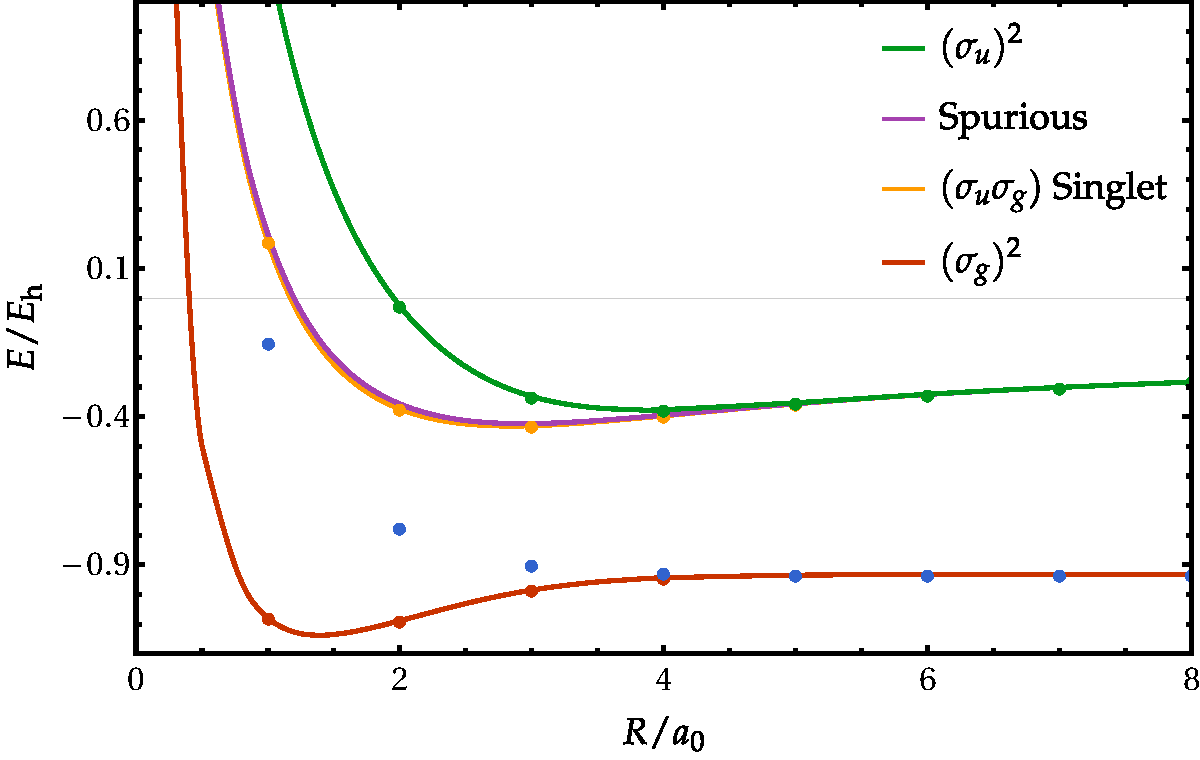
\includegraphics[width=\linewidth]{Figures/fig_1.pdf}
  \caption{
    OO-CID energies of \ce{H_2} in the STO-3G basis set with respect to the bond length $R$. The dots represent the corresponding FCI energies.
    \label{fig:fig_1}}
\end{figure}
%%% %%% %%% %%%

As even the smallest non-trivial CASSCF calculation is already quite messy, we start with a minimal MCSCF example to exemplify the flexibility of these ansatze.
We know that for the hydrogen molecule in a minimal STO-3G basis set \cite{Hehre_1969}, the two configuration interaction doubles (CID) energies correspond to the exact ground-state and doubly excited state within this basis.
The potential energy surfaces of these two states are plotted in Fig.~\ref{fig:fig_1} in orange and green line, the dots represent the corresponding FCI energies of this system.
The molecular orbitals of these two states are determined by the symmetry of the system, yet one can still rotate them and explore the orbital-optimized (oo) CID energy landscape in search of other stationary points.
In fact, we observe that there exists an oo-CID solution (see yellow curve in Fig.~\ref{fig:fig_1}), with the energy of the exact open-shell singlet which is usually unattainable by the CID ansätz.
This solution is associated with spatially symmetry-broken orbitals.
Unfortunately, there is also an additional spurious non-physical oo-CID solution (purple curve) which has also symmetry-broken orbitals.
The orbitals of the four solutions are given in the \SupInf.
This simple example shows that MCSCF ansatze are flexible enough to exhibit stationary points associated with physical states outside of their ``determinant space''.
In particular, in the following we will be interested in the description of excited states outside of the CAS by CASSCF wave functions.

\begin{table}
  \caption{Energies of \ce{H2} at $R=1~a_0$ using the 6-31G basis set for various formalism: FCI, SA-CASSCF with a (2,2) CAS, SA-CASSCF with a (3,2) CAS and SS-CASSCF with a (2,2) CAS.}
  \label{tab:tab_1}
  \begin{ruledtabular}
    \begin{tabular}{cccccc}
      spin & state & FCI  & SA(2,2) & SA(3,2) & SS(2,2) \\
      \hline
      \ce{Singlet}
           & 1 & -1.09897 & -1.07170 & -1.08924 & -1.09225 \\
           & Spurious &  &  &  & -1.08569 \\
           & Spurious &  &  &  & -1.07871 \\
           & 2 & -0.46395 & -0.43494 & -0.44196 & -0.46368 \\
           & 3 & -0.07450 &  & -0.06164 & -0.0594551 \\
           & 4 & 0.32015 & 0.33066 & 0.32624 & 0.31914 \\
           & Spurious &  &  &  & 0.31821 \\
           & Spurious &  &  &  & 0.31844 \\
           & Spurious &  &  &  & 0.32440 \\
           & 5 & 0.57224 &  & 0.61682 & 0.61429 \\
           & 6 & 0.86353 &  & 0.86876 & 0.86392 \\
           & Spurious &  &  &  & 0.85673 \\
           & Spurious &  &  &  & 0.86266 \\
           & Spurious &  &  &  & 0.86266 \\
           & 7 & 0.96373 &  &  & 0.91147 \\
           & 8 & 1.46479 &  &  & 1.45704 \\
           & 9 & 1.81277 &  &  & 1.80747 \\
           & 10 & 2.71948 &  &  & 2.71766 \\
           & Spurious &  &  &  & 2.70046 \\
           & Spurious &  &  &  & 2.69883 \\
      \hline
      \ce{Triplet}    
           & 1 & -0.57616 & -0.57166 & -0.57406 & -0.57417 \\
           & 2 & -0.28180 &  & -0.27990 & -0.27990 \\
           & 3 & 0.51519 &  & 0.51654 & 0.51638 \\
           & 4 & 0.62520 &  &  & 0.62401 \\
           & 5 & 1.30761 &  &  & 1.30572 \\
           & 6 & 1.61884 &  &  & 1.61685 \\
    \end{tabular}
  \end{ruledtabular}
\end{table}

%%% FIG 2  %%%
\begin{figure*}
  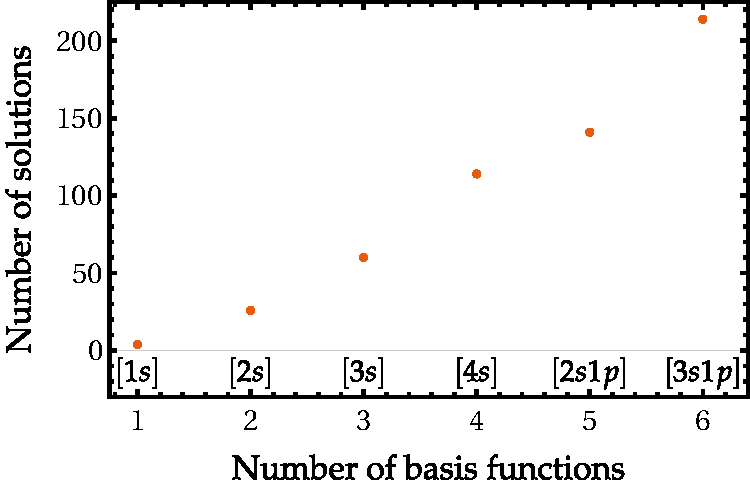
\includegraphics[width=0.3\linewidth]{Figures/fig_2a.pdf}
  \hspace{0.03\linewidth}
  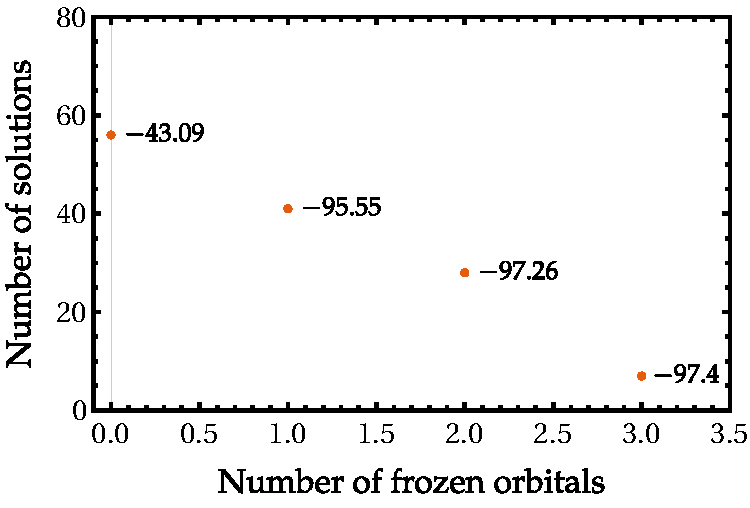
\includegraphics[width=0.3\linewidth]{Figures/fig_2b.pdf}
  \hspace{0.03\linewidth}
  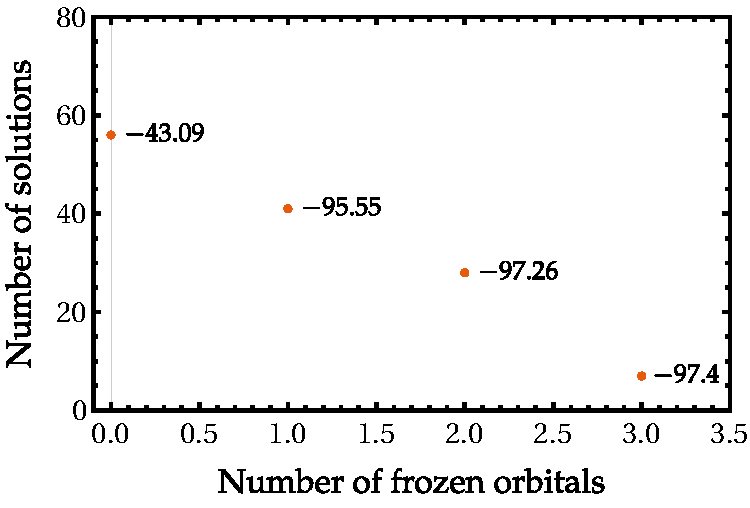
\includegraphics[width=0.3\linewidth]{Figures/fig_2c.pdf}
  \caption{Number of SS-CASSCF solution with respect to various parameters of the system. Left: Influence of the size of the basis set for \ce{H2} at $R=1~a_0$. Middle: Influence of the geometry for \ce{H2} in 6-31G basis set. Right: Influence of freezing core orbitals for the \ce{HF} molecule at $R=2~a_0$ in STO-3G basis set. \label{fig:fig_2}}
\end{figure*}
%%% %%% %%% %%%

Then, we turn to a slightly larger basis set, namely the 6-31G one, \cite{Ditchfield_1971} and consider a (2,2) CASSCF wave function.
Using SA-CASSCF one can obtain three singlet and one triplet state as shown in Table~\ref{tab:tab_1}.
On the other hand, using the same active space but in a SS formalism one can obtain an approximation of the sixteen FCI states of this system.
Table~\ref{tab:tab_1} shows that the agreement between the SS-CASSCF energies and their FCI counterparts is consistent for all states and is still quantitative outside of the CAS.
The mean absolute deviation is $0.00250~E_h$ for the four states within the CAS and $0.01106~E_h$ for the twelve remaining states.
In addition, as expected the SS (2,2) energies are in closer agreement than the SA (2,2) ones (which have a mean absolute deviation of $0.01782~E_h$), because the orbitals are fully optimized for each states.
Even with the only non-exact larger active space available, namely (3,2), the SA formalism cannot obtain as much states as the SS one with a (2,2) active space.

Because there is no free lunch, there is a counterpart to these advantages. Indeed, we can see that four singlet states exhibit close-lying spurious solutions (see Table~\ref{tab:tab_1}).
These four singlet states correspond to the singlet closed-shells of the system.
We should also mention that there may be more spurious solutions that have been missed by our grid-based search.
In order to design a SS-CASSCF algorithm, we need to understand where those spurious solutions originates from.
This is the aim of the next section.

%=================================================================%
\section{Origin of spurious solutions}
\label{sec:origin}
%=================================================================%

%%%%%%%%%%%%%%%%%%%%%%%%%%%%%%%%%%%%%%%%%%%%%%%%%%
\subsection{Influence of the system}
\label{sec:influence}
%%%%%%%%%%%%%%%%%%%%%%%%%%%%%%%%%%%%%%%%%%%%%%%%%%

Before looking in details into these spurious solutions, we look at the general trends of the number of solution with respect to some parameters of the system.
The left plot of Fig.~\ref{fig:fig_2} shows the number of solution with respect to the number of basis function per hydrogen atom for the hydrogen molecule at $R=1~a_0$.
The number of solution grows polynomially for the first four point.
Then we add basis functions with different symmetries therefore the growth is not smooth anymore, yet the number of solution is still increasing.
This shows that in real systems the number of solution should be expected to be really large.
Therefore, before working on a SS-CASSCF algorithm we should understand if this large number of solution is preocuppying or not.

It is now well-known that the number of solution in HF, DFT and CC is not constant with respect to variation of the geometry of the system. \todo{ref}
The middle plot of Fig.~\ref{fig:fig_2}, representing the number of solution of \ce{H2} in the 6-31G basis set, shows that the same behavior is observed in CASSCF theory.
Indeed, we can see that the number of solution is growing when the correlation is getting stronger, \ie when we stretch the bond.
We will investigate later one the potential energy curves of these solutions and the causes of appearance of additional solutions at large $R$.

Finally, we look at the influence of frozen core orbitals on the number of CASSCF solution.
The right plot of Fig.~\ref{fig:fig_2} shows the number of solution for the HF molecule at $R=2~a_0$ in the STO-3G basis set.
We see that the number of solution is decreasing each time we freeze one more orbital.
In addition, the energy of the highest solution (value in Hartree next to each dot) is also lower when core orbitals are frozen.
These two results were expected as the same trends were observed in the context of Hartree-Fock theory. \cite{Dong_2020}
We believe that one could take advantage of this property to target effectively core excited states at the SS-CASSCF level.

%%%%%%%%%%%%%%%%%%%%%%%%%%%%%%%%%%%%%%%%%%%%%%%%%%
\subsection{Index of the solutions}
\label{sec:geom}
%%%%%%%%%%%%%%%%%%%%%%%%%%%%%%%%%%%%%%%%%%%%%%%%%%

%%%  FIG 3  %%%
\begin{figure*}
  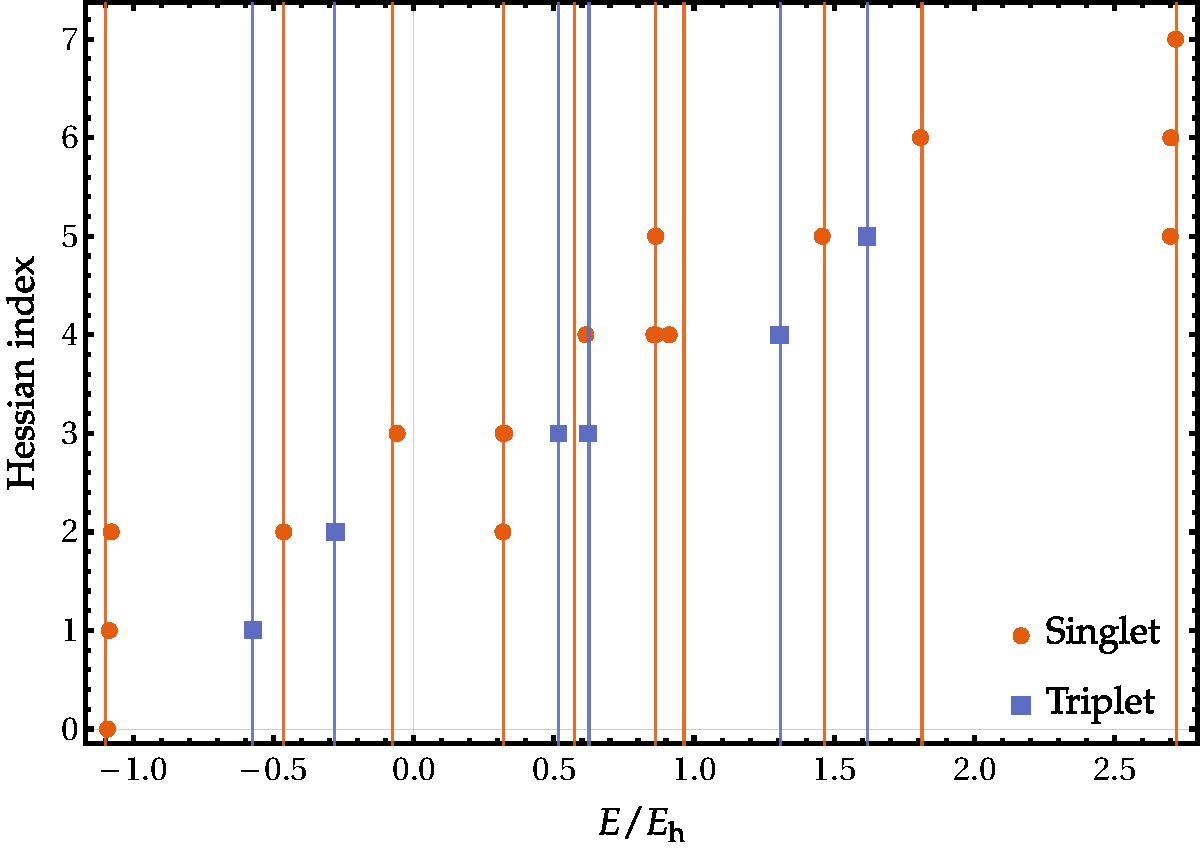
\includegraphics[width=0.4\linewidth]{Figures/fig_3a.pdf}
  \hspace{0.05\linewidth}
  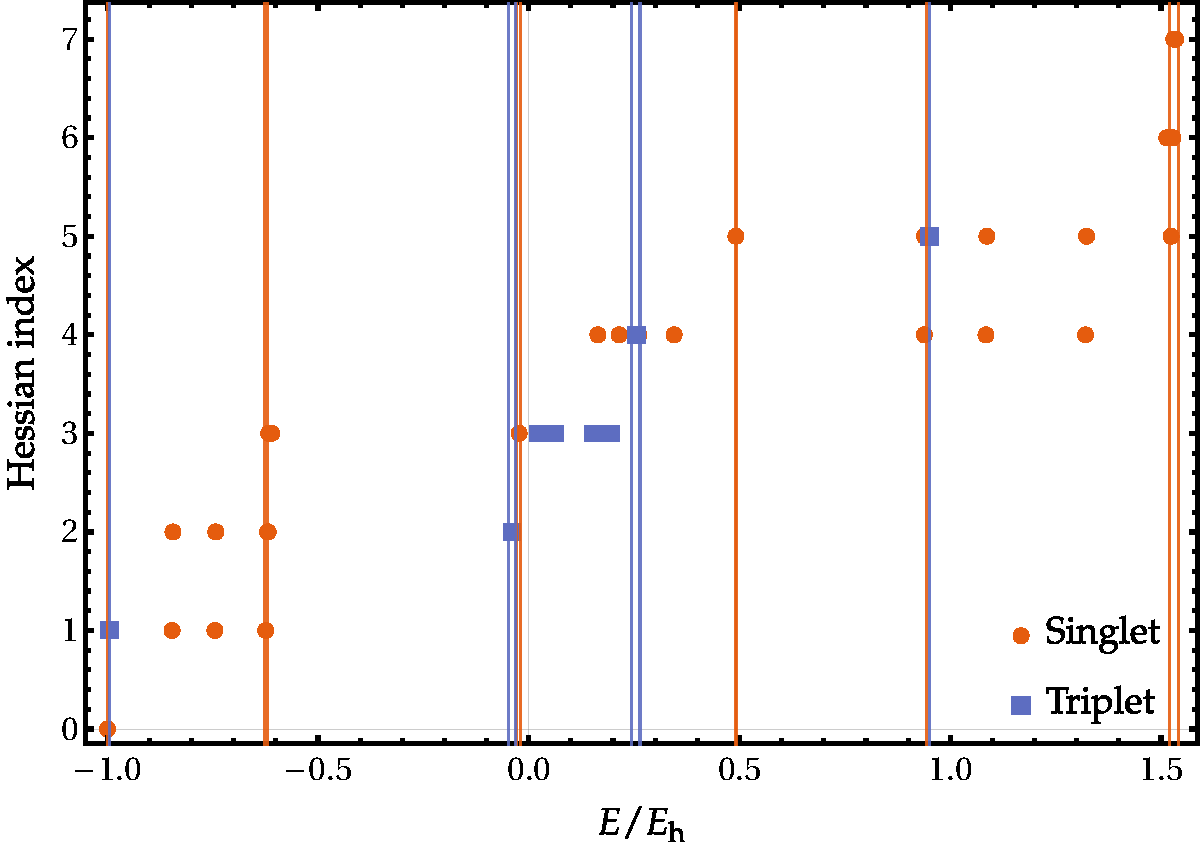
\includegraphics[width=0.4\linewidth]{Figures/fig_3b.pdf}
  \caption{Index of the SS-CASSCF solutions of \ce{H2} in the 6-31G basis set at $R=1~a_0$ (left) and $R=5~a_0$ (right) with respect to their energies
    \label{fig:fig_3}}
\end{figure*}
%%% %%% %%% %%%

The previous subsection has emphasized the need to understand the cause of these additional solutions.
The simplest characterization of CASSCF stationary points that one can use is the index of each stationnary point, \ie the number of negative eigenvalues of the hessian.
On the left plot of Fig.~\ref{fig:fig_3}, we can see the index of the solutions of Table~\ref{tab:tab_1} with respect to their energy.
We can see that close-lying spurious solutions may have different indexes.
For example, the three lowest solutions have indexes equal to 0, 1 and 2 in ascending order of energy.
At this stage, one can argue that in terms of energy spurious solutions are not that much worrying as each of them is fairly close to an FCI energy (vertical lines in  Fig.~\ref{fig:fig_3}).
\todo{Shall we add a sentence on variational upper bound?}

The right plot is the analog of the left one but in the strong correlation regime ($R=5~a_0$).
The first thing to notice is that now some spurious solutions are not close to any FCI energy.
Therefore one can argue that these solutions are much more preocuppying than what we have seen in the dynamic correlation regime.
However, all FCI energies remain approximately matched by at least one CASSCF solution.
So the problem of spurious solutions seems more serious in the strong correlation regime, which could have been expected as it has already been observed in the HF and CC contexts. \todo{ref}

%%%%%%%%%%%%%%%%%%%%%%%%%%%%%%%%%%%%%%%%%%%%%%%%%%
\subsection{Natural orbitals and symmetry-broken solutions}
\label{sec:natural}
%%%%%%%%%%%%%%%%%%%%%%%%%%%%%%%%%%%%%%%%%%%%%%%%%%

%%%  FIG 4  %%%
\begin{figure*}
  \begin{subfigure}[b]{0.31\textwidth}
    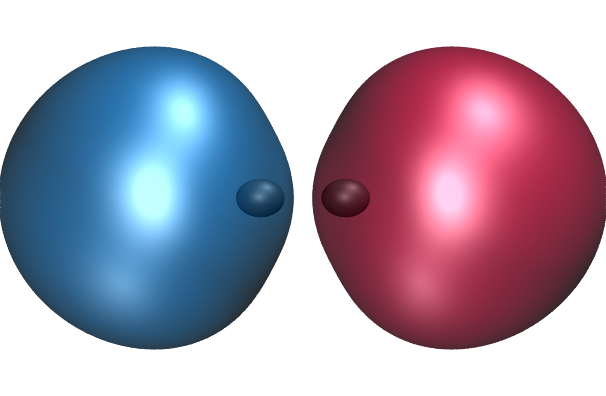
\includegraphics[width=0.5\textwidth]{Figures/h2_HF_mo2.cube.png}
    \subcaption*{\centering $(1\sigma_u)~n_\text{occ}~=~0.011$}
    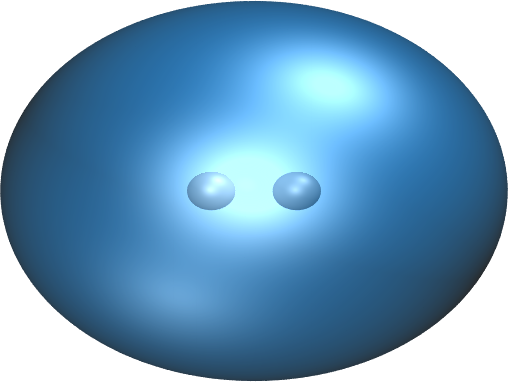
\includegraphics[width=0.5\textwidth]{Figures/h2_HF_mo1.cube.png}
    \subcaption*{\centering $(1\sigma_g)~n_\text{occ}~=~1.989$ \protect\\ $E=-1.09225~E_h$}
  \end{subfigure}
  \begin{subfigure}[b]{0.31\textwidth}
    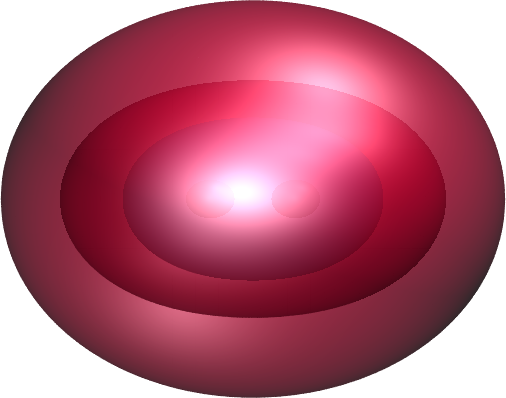
\includegraphics[width=0.5\textwidth]{Figures/h2_HF_mo3.cube.png}
    \caption*{\centering $(2\sigma_g)~n_\text{occ}~=~0.007$}
    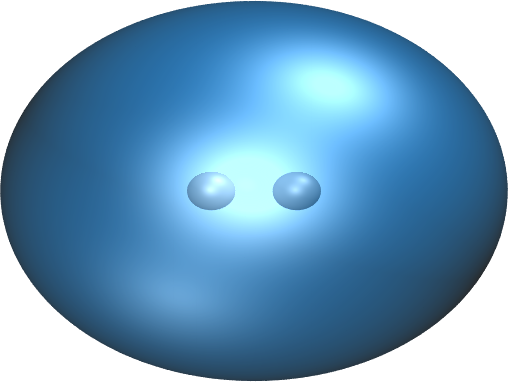
\includegraphics[width=0.5\textwidth]{Figures/h2_HF_mo1.cube.png}
    \caption*{\centering $(1\sigma_g)~n_\text{occ}~=~1.993$ \protect\\ $E=-1.08569~E_h$}
  \end{subfigure}
  \begin{subfigure}[b]{0.31\textwidth}
    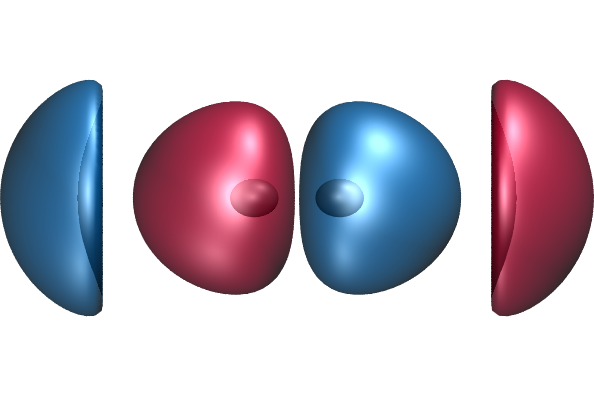
\includegraphics[width=0.5\textwidth]{Figures/h2_HF_mo4.cube.png}
    \caption*{\centering $(2\sigma_u)~n_\text{occ}~=~0.0002$}
    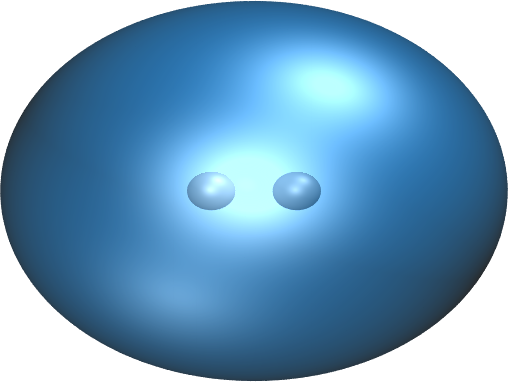
\includegraphics[width=0.5\textwidth]{Figures/h2_HF_mo1.cube.png}
    \caption*{\centering $(1\sigma_g)~n_\text{occ}~=~1.9998$ \protect\\ $E=-1.07871~E_h$}
  \end{subfigure}
  \caption{Natural orbitals of the three lowest (2,2) SS-CASSCF singlet solutions of \ce{H2} at $R=1~a_0$ \label{fig:fig_4}}
\end{figure*}
%%% %%% %%% %%%

Now, we would like to understand in details the difference between close-lying solutions in order to shed light on the physical phenomena causing the appearance of these spurious solutions.
To do this, we start by focusing on the two spurious solutions lying close to the ground state for the hydrogen molecule in the 6-31G basis set (see Table~\ref{tab:tab_1}).
Figure~\ref{fig:fig_4} shows the natural orbitals (in the active space) and their occupancy for these three solutions.
Because there are only two orbitals in the active space, only two orbitals can have a non-zero occupation.
We know that at $R=1~a_0$ the HF ground state, corresponding to a single determinant with two electrons in the $(1g)$ orbital, is a reasonable approximation of the FCI ground state.
We can see that these three solutions have almost two electrons in the $(1g)$ orbital which is in agreement with the performance of HF.
The difference between these solutions is the orbital in which the remaining small fractional occupation is put.
The three solutions correspond to the three possible choices of virtual orbital to be put in the active space.
We observe the same phenomenon for the three other closed-shell states.
In each case, we have a dominant single configuration correlated by one of the three other remaining orbitals.
For the two intermediate closed-shell states the fourth closely-lying solution correspond to a symmetry-broken solution.
In both cases, the symmetry-broken solution is the closest to the FCI energy among the four solutions.

%%%  FIG 5  %%%
\begin{figure}
  \centering
  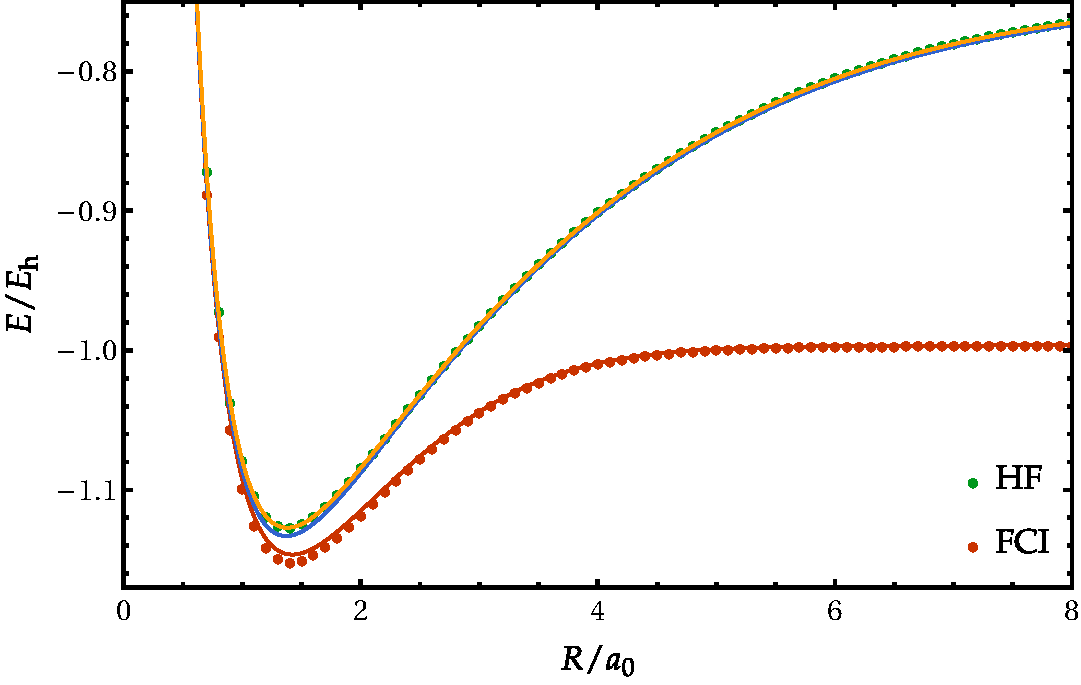
\includegraphics[width=0.9\linewidth]{Figures/fig_5.pdf}
  \caption{Potential energy curves of the three lowest (2,2) SS-CASSCF singlet states (lines) for \ce{H2} in the 6-31G basis set (see Tab.~\ref{tab:tab_1}). The dots correspond to the FCI and HF ground states. \label{fig:fig_5}}
\end{figure}
%%% %%% %%% %%%

Now we investigate the behavior of these solutions when the bond is stretched.
In Fig.~\ref{fig:fig_5} we can see that only one of these solutions goes to the correct dissociation limit.
This solution is the lowest one at $R=1~a_0$ and have a fractional occupation in the $(1\sigma_u)$ orbital (see Fig.~\ref{fig:fig_4}).
At dissociation, the configuration of this solution is $1(\sigma_g)1(1\sigma_u)$.
On the other hand, the two other solutions configuration are $1.997(1\sigma_g)0.003(2\sigma_g)$ and $1.999(1\sigma_g)0.001(2\sigma_u)$, respectively.
This is due to the fact that the additional active orbital does not have the required symmetry to mix with the $(1g)$ orbital to produce the correct dissociation limit.
Therefore, these solutions have an energy slightly below the HF dissociation limit as they recover only a small part of the correlation energy.
So we can already say that some spurious solutions completely off from FCI energies in Fig.~\ref{fig:fig_3} correspond to wrong HF dissociation limits.

%%%  FIG 6  %%%
\begin{figure}
  \centering
  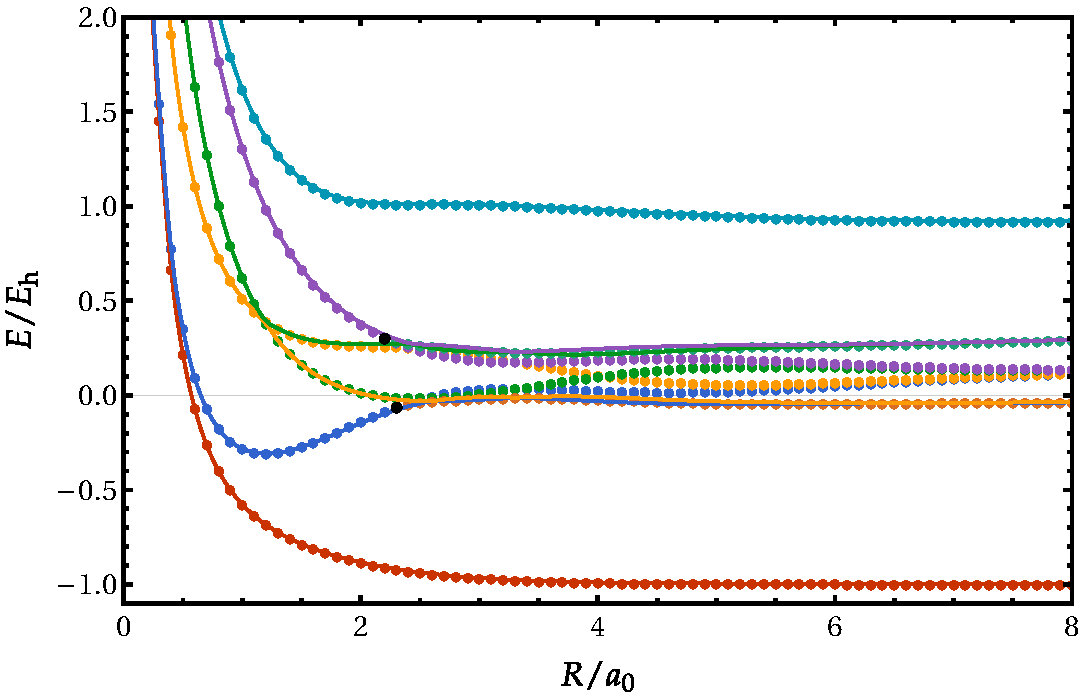
\includegraphics[width=0.9\linewidth]{Figures/fig_6.pdf}
  \caption{Potential energy curves of the (2,2) SS-CASSCF triplet states of \ce{H2} in the 6-31G basis set. \label{fig:fig_6}}
\end{figure}
%%% %%% %%% %%%

At this point we still need to understand the origin of the additional solutions appearing in the strong correlation limit.
To investigate this we plot the potential energy curves of the (2,2) SS-CASSCF triplet states of the system, see Fig.~\ref{fig:fig_6}.
We have seen that at equilibrium there are six CASSCF triplet solutions which are all good approximations of one of the six FCI triplets.
However, one can see in Fig.~\ref{fig:fig_6} that the four intermediate solutions are going to the same wrong dissociation limit (see the four FCI dissociation limits represented by the dots).
On the other hand, the lowest and highest triplets are in agreement with their FCI counterpart at all bond lengths.
At $R\simeq 2.3~a_0$ and $R\simeq 2.4~a_0$ (black dots), two additional triplet CASSCF solutions appear and these solutions go to the two correct dissociation limits (orange and light green dots).
These two solutions are spin pure ($S^2=2$) but their natural orbitals are spatially symmetry-broken (see \SupInf).
So these black dots correspond to CASSCF Coulson-Fisher points. \todo{Has it already been observed? Read thoroughly biblio}

The situation for the six open-shell singlets is completely analog, \ie the four intermediate solutions at $R=1~a_0$ go to some wrong dissociation limit and two spatially symmetry-broken open-shell singlets appear.
The corresponding potential energy surfaces and natural orbitals are given in the \SupInf.
Therefore, one source of additional solutions in the strong correlation regime is symmetry breaking which is completely analog to what is observed in HF. \todo{ref}
However, because the CASSCF ans\"atz is much more flexible than one single determinant, CASSCF symmetry breaking should be less common than in HF.

Finally, we need to discuss the behavior of the three higher closed-shell solutions.
For the symmetry-adapted solutions (three per closed-shell, see Fig.~\ref{fig:fig_4}) this is analog to the case of the ground state discussed in details above (see Fig.~\ref{fig:fig_5}), \ie only one solution out of the three close-lying ones is going to the corresponding correct dissociation limit.
The two spatially symmetry-broken closed-shell found at $R=1~a_0$ also evolve to the correct dissociation limit.
For the second closed-shell excited state (state 6 in Table~\ref{tab:tab_1}), we have found a degenerate spin-symmetry broken solution.
In fact, the corresponding exact solution is degenerate with a triplet at dissociation limit.
So the spin symmetry-broken solution correspond to a combination of these degenerate singlet and triplet.
Degeneracy of a singlet and a triplet state at dissociation yielding the possibility to converge on a spin symmetry-broken mix is also a cause of additional SS-CASSCF solutions.

Close to the first and third closed-shell excited state (states 4 and 10) we have also found several spatially symmetry-broken solutions with a dominant single-determinant configuration.
This is consistent with the fact that HF can describe these two dissociation limits with one spatially symmetry-broken single determinant. \todo{Do we have a ref for this? First year PhD report?}
In addition, the CASSCF ans\"atz can represent these two states in an alternative way without resorting to symmetry-breaking.
Indeed, by putting the two electrons in two different orbitals, SS-CASSCF can represent these two anti-bonding closed-shells (see \SupInf~for the corresponding natural orbitals).
These two ways of representing the same state gives the last cause of appearance of additional solutions in the strong correlation regime in this system.

%%%%%%%%%%%%%%%%%%%%%%%%%%%%%%%%%%%%%%%%%%%%%%%%%%
\subsection{Spurious solutions in larger system}
\label{sec:largersystem}
%%%%%%%%%%%%%%%%%%%%%%%%%%%%%%%%%%%%%%%%%%%%%%%%%%

At this stage, we believe that we have a quite exhaustive picture of the solution space of \ce{H2} in the 6-31G basis set.
Of course, one need to understand how does this solution space evolves when the basis set is increased and when we add more orbitals to the active space if we want conclusions about the solution space to be useful in practice.
Firstly, we consider again the \ce{H2} molecule at $R=1~a_0$ with a (2,2) CAS but in the slightly larger 6-311g basis set (three basis function per hydrogen atom). \todo{ref}
We find that in this case there are five close-lying ground-state solutions, the energies of these states are given in Table~\ref{tab:tab_2}.
From what we have seen before (see Fig.~\ref{fig:fig_4}), this was expected as there are five possible virtual orbitals that can be put in the (2,2) active space to correlate the HF ground-state determinant.
Higher in the spectrum, we find five other groups of five or six close-lying solutions, which correspond to the five remaining closed-shell states.
The sixth state, when present, corresponds to a symmetry-broken solution as observed in the smaller 6-31g basis set.
Therefore, because spurious solutions correspond to different possible choices for orbitals in the active space, the number of such solutions is going to grow combinatorially with respect to the size of the basis set.

\begin{table}[h!]
  \caption{Ground-state (2,2) SS-CASSCF energies of \ce{H2} at $R=1~a_0$ using the 6-311G basis set and its FCI counterpart.}
  \begin{ruledtabular}
    \label{tab:tab_2}
    \begin{tabular}{clllll}
      FCI & -1.10267 & & & &\\
      \hline
      SS(2,2) & -1.09429 & -1.08866 & -1.08074 & -1.08033 & -1.08026
    \end{tabular}
  \end{ruledtabular}
\end{table}

To further illustrate this result, we consider a larger active space. Table~\ref{tab:tab_3} shows the (3,2) SS-CASSCF solutions for the four lowest FCI states of \ce{H2} at $R=1~a_0$ using the 6-31G basis set.
There are two spurious solutions lying close to the ground state.
The three solutions correspond to the three possible choices of two virtual orbitals out of three to fill out the active space.
For the first excited closed-shell state we have found the three solutions analog to the ones of the ground state.
We have not found a symmetry-broken solution for this state as in the case of the (2,2) active space (see Table~\ref{tab:tab_1}).
Our grid-based approach may have missed this solution or this larger active space might give enough flexibility so that breaking the symmetry is not needed.

Now turning to the open-shell singlets, which do not exhibit close-lying spurious solutions when one use two active orbitals.
An open-shell state need for a proper minimal description at least two orbitals, one for each electron.
Therefore if the active space contain only two orbitals there is no freedom in the choice of orbitals once the two singly-occupied active orbitals have been chosen.
On the other hand, adding an orbital to the active space gives a freedom in the choice of the virtual orbital to add to the active space to correlate the open-shell, resulting in close-lying open-shell solutions.
Table~\ref{tab:tab_3} shows that indeed the open-shell states also exhibit close-lying spurious solutions when the active space is enlarged.

\begin{table}
  \caption{Four lowest FCI states of \ce{H2} at $R=1~a_0$ using the 6-31G basis set and their (3,2) SS-CASSCF counterpart.}
  \begin{ruledtabular}
    \label{tab:tab_3}
    \begin{tabular}{cllll}
      state & 1  & 2 & 3 & 4 \\
      \hline
      FCI & -1.09897 & -0.46395 & -0.07450 & 0.32015 \\
      \hline
      SS(2,2) & -1.09225 & -0.46368 & -0.0594551 & 0.31914 \\
            & -1.08569 &  &  & 0.31821 \\
            & -1.07871 &  &  & 0.31844 \\
            &  &  &  & 0.32440 \\
      \hline
      SS(3,2) & -1.09875 & -0.463822 & -0.0711398 & 0.315896 \\
            & -1.09256 & -0.463689 & -0.0632185 & 0.320249 \\
            & -1.08581 &  & -0.0594551 & 0.322577 \\
    \end{tabular}
  \end{ruledtabular}
\end{table}

%%%%%%%%%%%%%%%%%%%%%%%%%%%%%%%%%%%%%%%%%%%%%%%%%%
\section{Avoided crossing}
\label{sec:avoided}
%%%%%%%%%%%%%%%%%%%%%%%%%%%%%%%%%%%%%%%%%%%%%%%%%%

In this last section we will investigate the description of avoided crossings by SS-CASSCF.
It has been shown that HF solutions behave ``quasi-diabatically'' in the vicinity of avoided crossings. \cite{Thom_2009}
One can recover the avoided crossing by making the HF solutions interact through the Hamiltonian, resulting in a non-orthogonal (NO) CI scheme. \cite{Burton_2019}
Therefore, it will be interesting to see if SS-CASSCF solutions also behave ``quasi-diabatically'' or if they can reproduce the avoided crossing.
To answer this question we investigate the LiF molecule in the STO-3G basis set.
Indeed, the ionic ground state of this molecule at equilibrium undergoes an avoided crossing with a covalent excited state when the bond is stretched. \cite{Thom_2009,Mahler_2021} \todo{Add some ref}

We start by focusing on the sole ground-state.
The ground-state is a closed-shell ionic state at equilibrium and it dissociates to two open-shell atom.
At equilibrium the HF ground-state gives a fairly good description of this closed-shell state.
However, this HF solution cannot describe the correct dissociation limit. \todo{add ref}
Figure~\ref{fig:fig_7} shows the lowest (2,2) SS-CASSCF singlet solutions (lines) as well as the three lowest FCI singlets (dots).
The SS-CASSCF ground-state solution at equilibrium (red curve) correspond to a dynamically correlated HF ground state, \ie the active space contains the HF highest occupied MO, a $\pi_y$ orbital mostly localized on the fluorine atom, and the associated $\pi_y^*$.
By delocalizing a small fraction of electron in the $\pi_y^*$ orbital the SS-CASSCF solution achieve some resonance stabilization between the HF ground state and the singlet charge-transfer excited state.
However, this solution is going to the wrong dissociation limit as we can see on the plot.

We have found another minimum solution at dissociation limit (green curve).
This solution correspond to the two open-shell atom, the active space has one electron in the $2s$ of the lithium atom and one electron in the $\pi_z$ localized on the fluorine.
When $R$ decrease the electron in the $2s$ is transfered to the $\pi_z$ and at equilibrium this solution is equivalent to the closed-shell HF ground state.
The $2s$ orbital localized on the Lithium atom does have the correct symmetry to dynamically correlate the HF determinant as the $1 {}^1\Sigma^+_{\text{eq}}$.

Now turning to the SS-CASSCF description of the avoided crossing.
Figure~\ref{fig:fig_7} shows that the CASSCF singlet states are behaving in a ``quasi-diabatic'' manner. The two singlet excited states (yellow and purple curves) are dissociating to the lowest dissociation limit while one of them should interact with the ground-state to form an avoided crossing.
It would be interesting to make these three solutions interact through the Hamiltonian in analogy with NOCI.
By scrutinizing the symmetry of the natural orbitals of the two singlet excited states, we expect that only one of them can interact with the ground state (see \SupInf).
It would also be interesting to see if one can describe the ground state at all bond lengths by interaction of the $1 {}^1\Sigma^+_{\text{eq}}$ and $1 {}^1\Sigma^+_{\text{diss}}$ solutions correct at small and large $R$, respectively.
We keep this for a future work.

%%%  FIG 7  %%%
\begin{figure}
  \centering
  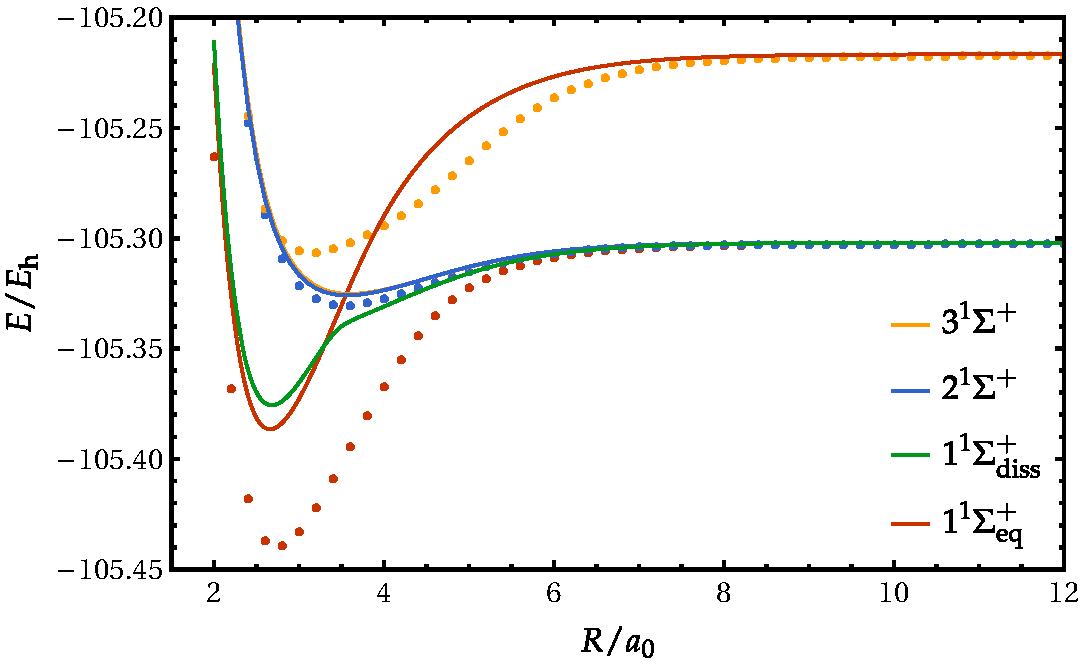
\includegraphics[width=0.9\linewidth]{Figures/fig_7.pdf}
  \caption{Potential energy curves of the SS-CASSCF states of \ce{LiF} in the STO-3G basis set. \label{fig:fig_7}}
\end{figure}
%%% %%% %%% %%%

%=================================================================%
\section{Conclusion}
\label{sec:conclusion}
%=================================================================%

\todo{Add conclusion}

%%%%%%%%%%%%%%%%%%%%%%%%
\begin{acknowledgements}
%%%%%%%%%%%%%%%%%%%%%%%%
\todo{Add acknowledgements}
%%%%%%%%%%%%%%%%%%%%%%
\end{acknowledgements}
%%%%%%%%%%%%%%%%%%%%%%

\appendix

%%%%%%%%%%%%%%%%%%%%%%%%%%%%%%%%%%%%%%
\section{Gradient and hessian matrix elements}
\label{app:appendixA}
%%%%%%%%%%%%%%%%%%%%%%%%%%%%%%%%%%%%%%

In this appendix we give explicit expressions to compute the gradient and hessian used in the Newton-Raphson algorithm.
The gradient can be divided in two parts, namely the CI part $g^c$ and the orbital part $g^o$.
This latter can be divided further in three parts corresponding to the non-redundants rotations for a CASSCF wave function: core-active, core-virtual and active-virtual.

\begin{align}
  \label{eq:CASSCF_CI_Gradient}
  g^c_{K} &= \eval{\mleft(\pdv{E}{S_{K}}\mright)}_{\bm{\lambda}=0} = \mel**{\Psi_0}{\com{\hH}{\hS}}{\Psi_0} \\
          &= 2\mel**{\Psi_K}{\hH}{\Psi_0} \notag \\
          &= 2\sum_{IJ}C_{K,I}^*\mel{I}{\hH}{J}C_{0,J} \notag
\end{align}

\begin{equation}
  \label{eq:CASSCF_Orb_Gradient_general}
  g^o_{pq} = \eval{\mleft(\pdv{E}{\kappa_{pq}}\mright)}_{\bm{\lambda}=0} = \mel**{\Psi_0}{\com{\hH}{\hK}}{\Psi_0}
\end{equation}

\begin{subequations}
  \label{eq:CASSCF_Orb_Gradient}
  \begin{align}
    g^o_{ai} &= 4(\FC{ai} + \FA{ai}) \\
    g^o_{ti} &= 4(\FC{ti} + \FA{ti}) - 2\sum_v \gamma_{tv}\FC{iv} -4\sum_{vxy}\Gamma_{tvxy}\braket{ix}{vy} \\
    g^o_{at} &= 2\sum_v \gamma_{tv}\FC{av} + 4\sum_{vxy}\Gamma_{tvxy}\braket{ax}{vy}.
  \end{align}
\end{subequations}
where we have introduced the core and active parts of the generalized Fock matrix
\begin{align}
  \label{eq:CoreActGeneralizedFock}
  \FC{pq} &= h_{pq} + \sum_{i} 2\ceri{pq}{ii} - \ceri{pi}{iq} \\
  \FA{pq} &= \sum_{vx}\gamma_{vx}(\ceri{pq}{vx} - \frac{1}{2}\ceri{px}{vq})
\end{align}

Similarly, we can divide the hessian in three parts: CI-CI $H^{cc}$, Orb-Orb $H^{oo}$ and Orb-CI $H^{oc}$. The CI-Orb part is equivalent to the latter up to a transposition.

\begin{align}
  \label{eq:CASSCF_CICI_Hessian}
  H^{cc}_{K,L} &= \eval{\mleft(\pdv{E}{S_{K}}{S_{L}}\mright)}_{\bm{\lambda}=0} = \mel**{\Psi_0}{\com{\com{\hH}{\hS}}{\hS}}{\Psi_0} \\
  &= 2\mel**{\Psi_K}{\hH - E_0}{\Psi_L} \notag \\
  &= 2\sum_{IJ}C_{K,I}^*\mel**{I}{\hH}{J}C_{L,J} - E_0\delta_{K,L} \notag
\end{align}

\begin{align}
  \label{eq:CASSCF_OrbCI_Hessian}
  H^{oc}_{pq,K} &= \eval{\mleft(\pdv{E}{\kappa_{pq}}{S_{K}}\mright)}_{\bm{\lambda}=0} = \mel**{\Psi_0}{\com{\com{\hH}{\hK}}{\hS}}{\Psi_0} \\
                &= \mel**{\Psi_K}{\com{\hH}{E_{pq}^-}}{\Psi_0} \notag \\
                &= 2\sum_{IJ}C_{K,I}^*\mel{I}{\com{\hH}{E_{pq}^-}}{J}C_{0,J} \notag
\end{align}
where we have introduced $E_{pq}^- = \cre{p}\ani{q} - \cre{q}\ani{p}$ the anti-symmetrized spin-averaged excitation operator.
\begin{align}
  \label{eq:MCSCF_SO_OrbOrb_Hessian}
  H^{oo}_{pq,rs} &= \eval{\mleft(\pdv{E}{\kappa_{pq}}{\kappa_{rs}}\mright)}_{\bm{\lambda}=0} = \mel**{\Psi_0}{\com{\com{\hH}{\hK}}{\hK}}{\Psi_0} \\
                   &= \frac{1}{2}(1+P_{pq,rs})\mel**{\Psi_0}{\com{\com{\hH}{E_{pq}^-}}{E_{rs}^-}}{\Psi_0} \notag
\end{align}

%%%%%%%%%%%%%%%%%%%%%%
\bibliography{MCSCF_LSP}
%%%%%%%%%%%%%%%%%%%%%%

\end{document}
